\documentclass[../main.tex]{subfiles}

\begin{document}

\problem{3}

\problempart{a}

Briefly describe why scramjets (theoretically) solve some of the specific issues that ramjets encounter at higher Mach numbers.

\discussion{}
Scramjets follow the same foundational principles as ramjets with the added caveat that they are capable of supersonic combustion.
The need to slow the flow through the ramjet to subsonic velocities adds significant losses at higher Mach numbers.
By utilizing supersonic combustion, the compression and velocity reduction in the flow can be performed solely through oblique shocks which are more efficient than normal shocks.
This enables air-breathing propulsion at higher Mach numbers than ramjets are capable of supporting, and therefore allows a vehicle to expand its flight envelope and Mach regime.
Another issue seen in ramjets at high Mach is the static temperature experienced in the combustion region.
As cruise Mach and shock strength increase, the static temperature of the flow grows dramatically.
Adding heat to such high-temperature flows reduces the effective amount of thrust that can be extracted from the propulsion system. 
A scramjet system does not generate static temperatures as high as a ramjet for the given Mach number because there is no need to introduce a normal shock to the flow.
In addition to the thrust aspect, limiting the temperature experienced in the flowpath alleviates stress on the vehicle's material requirements and thermal management systems.
Despite the lack of moving parts, both ramjets and scramjets are incredibly complex propulsion systems due to the highly complicated flow physics and thermal environments encountered in high supersonic or hypersonic flows.


\problempart{b}

How do the inlet freestream pressure ratio, inlet total pressure ratio, and combustor inlet freestream temperature compare for this scramjet design compared to the ramjet (with spike) design? 
You must actually calculate the numbers. 
Does this support what you said in part (a)?

\assumptions{}
Both the ramjet and scramjet are experiencing identical freestream conditions with \(M_\infty=5,\, p_\infty=20\,\unit{\kilo\pascal},\, \textrm{and}\,T_\infty=217\,\unit{\kelvin}\).
The ramjet has a 21 degree inlet spike half angle, per Problem 2.
The assumptions used for Problem 2 are maintained here for use in isentropic relations and normal/oblique shock calculations.

\solution{}

The solution methodology for the scramjet case is outlined below.
For brevity, not all calculations are shown.
\textit{Note: All calculations performed in Python, see Appendix \ref{Problem3Python}}.

\begin{enumerate}

    \item Numerically solve for the shock angle \(\beta\) with \(M_\infty=5\) and \(\theta=7^\circ\). (Polarity of the shock angle does not impact the solution process so for simplicity we take the positive value.)

    \item With \(\beta\), solve for the normal component of the freestream Mach number and use normal shock relationships to determine the normal component of the post-oblique shock flow.

    \item Solve for \(M_2\) using \(\beta\) and \(\theta\).
    
    \item Recognize that the second oblique shock is generated by a turn angle of \(\theta=7^\circ\), solve for the second \(\beta\) using \(M_2\) and \(\theta\).
    
    \item As before, solve for the component of \(M_2\) normal to the second oblique shock, \(M_{2n'}\), then find \(M_3\).

    \item Given \(M_1, M_{1n}, M_{2n}, M_2, M_{2n'}, \,\textrm{and}\, M_3\), isentropic and normal shock relationships can be used to solve for the inlet freestream pressure ratio, the inlet total pressure ratio, and the combustor inlet static temperature.
        The procedure used in Problem 2 is repeated for many of the calculations shown here.

\end{enumerate}

We now solve for the scramjet inlet freestream pressure ratio, the inlet total pressure ratio, and the combustor inlet static temperature using the above procedure.
Results from Problem 2 are used to compare the ramjet performance at the same \(M_\infty=5\) condition.
Table \ref{table} compares the two propulsion systems.

\begin{table}[h!]
    \begin{tabular}{|ll|ll|ll|}
    \hline
    \multicolumn{2}{|c|}{\textbf{Inlet Static Pressure Ratio}} & \multicolumn{2}{c|}{\textbf{Inlet Total Pressure Ratio}} & \multicolumn{2}{l|}{\textbf{Combustor Inlet \(T_\infty\) {[}K{]}}} \\ \hline
    \multicolumn{1}{|l|}{Ramjet}           & Scramjet          & \multicolumn{1}{l|}{Ramjet}          & Scramjet          & \multicolumn{1}{l|}{Ramjet}                   & Scramjet                 \\ \hline
    \multicolumn{1}{|l|}{74.30}            & 4.55              & \multicolumn{1}{l|}{0.16}            & 0.92              & \multicolumn{1}{l|}{1244.75}                  & 343.04                   \\ \hline
    \end{tabular}
    \caption{Ramjet vs. Scramjet Performance at \(M_\infty=5\).}
    \label{table}
\end{table}

The results in table \ref{table} support the discussion in part (a). 
The ramjet inlet has a static compression ratio over 16x that of the scramjet, with a total pressure ratio approximately 1/6\textsuperscript{th} that of the scramjet. 
Despite the scramjet's reduced static compression, the overall efficiency of the propulsion system as measured by total pressure ratio is significantly larger.
The combustor inlet temperature is also significantly smaller, approximately 25\% of the ramjet value.
The reduced combustor static temperature enables more thrust to be pulled out of the working fluid in the scramjet.

\problempart{c}

Under these conditions, what is the Mach number of the flow at the inlet of the combustor? 
What combustion challenges do we face in efficiently burning fuel at this Mach number?

\solution{}
With \(p_{t,3}\) and \(p_3\), the Mach number at the inlet of the combustor, \(M_3\), can be calculated using isentropic relations.
\[
    M_3 = \sqrt{
        \left[{\left(\frac{p_{t,3}}{p_3}\right)^\frac{\gamma}{\gamma-1} - 1}\right] \frac{2}{\gamma-1}
    }
\]

\[
    M_{combustor} = 3.74
\]

Burning fuel at high Mach numbers is difficult for several reasons, some of which inclue flame dynamics, fuel-air mixing, and residence time.
Keeping a flameholder operating effectively in such extreme conditions is difficult, a problem exacerbated by the difficulty in thoroughly mixing the fuel and the air going through the combustor to ensure uniform combustion and flow properties.
A packet of air moving through a combustor at Mach 3.74 is only exposed to the flameholder and fuel injection for a scant amount of time.
Getting good combustion in such a small window of time is a highly complex problem that is still an active research area.

\problempart{d}

Let's now investigate the qualitative effect of viscosity on shock reflections.
We will focus our attention to the last reflected shock before the fuel-injection site.
An effect of viscosity is to decelerate the flow in the vicinity of the wall such at \(u_{wall}=0\).
We will assume that the scramjet is a height of \(H\) from the bottom wall to the top wall.
We will also assume that u is equal to its local freestream value a distance \(\delta\) away from the walls.
Sketch \(y\) versus \(\beta\) for \(0<y<H\).
In addition, sketch the more realistic shape of the shock.

\discussion{}

Inclusion of viscous effects changes the way that shocks propogate throughout a flowpath.
Because of the non-slip condition with \(u_{wall}=0\), the shock strength required to turn the flow near the wall is smaller and therefore the shock angle \(\beta\) near the wall is also smaller.
Figure \ref{y_vs_beta} shows a qualitative sketch of the \(y\) vs. \(\beta\) distribution from the bottom surface of the inlet to the top along the reflected oblique shock.
Similar to the velocity profile, \(\beta\) begins at 0 and increases until the freestream value of \(\beta\) is reached at a height off of the wall of \(\delta\).
The shock angle is constant with freestream velocity until a height of \(H-\delta\) where the upper surface boundary layer begins to influence the flow.
The shock angle then decreses back to a value of 0 at the upper wall.

\begin{figure}[h!]
    \centering
    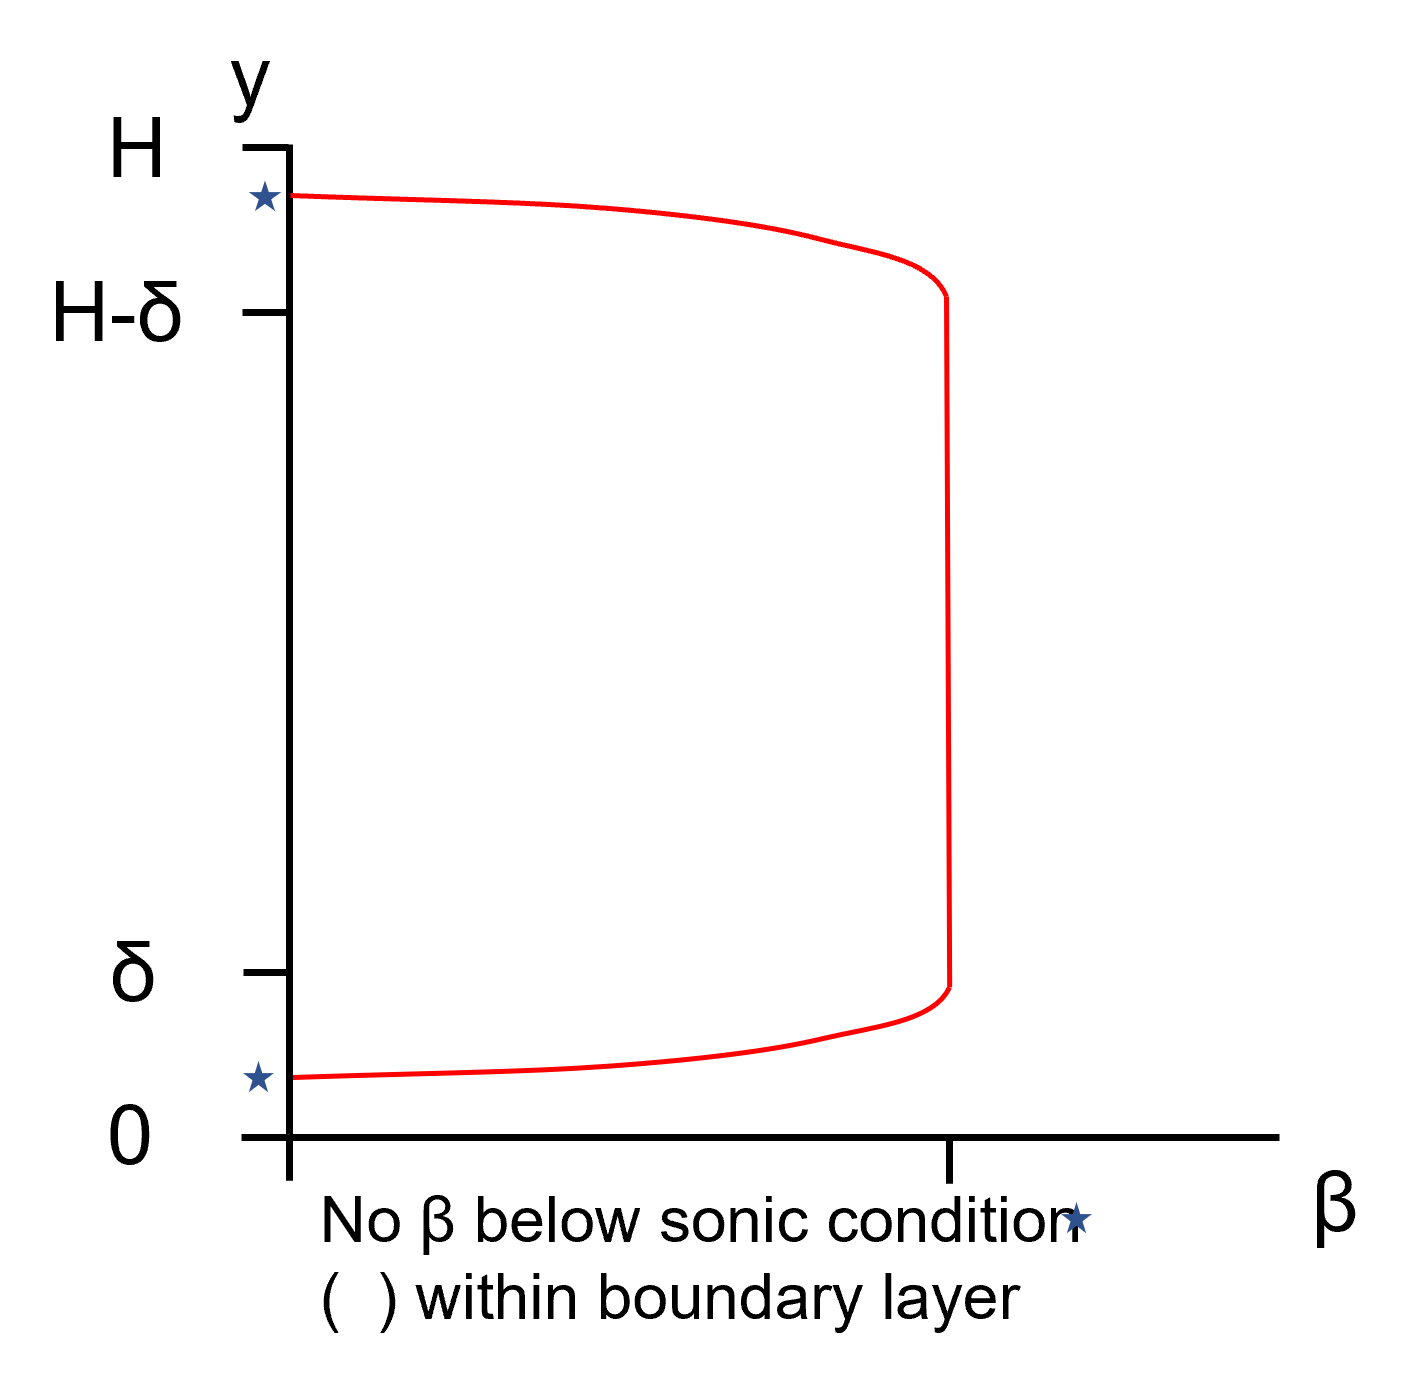
\includegraphics[scale=1.0]{../../images/problem_3/y_vs_beta.png}
    \caption{y vs. \(\beta\)}
    \label{y_vs_beta}
\end{figure}

Figure \ref{viscous_inlet} shows a sketch of the scramjet inlet region with both reflected shocks and viscous effects included.
Using knowledge from figure \ref{y_vs_beta} allows us to sketch what happens to the shock in the region near the wall in the viscous boundary layer.
The shock is concave on the bottom surface until a height of \(\delta\) and convex on the top surface from \(H-\delta\) to \(H\).
The finer details of the shockwave-boundary layer interactions are neglected here but the high-level qualities of the boundary layer's impact on the shockwave are represented qualitatively.

 
\begin{figure}[h!]
    \centering
    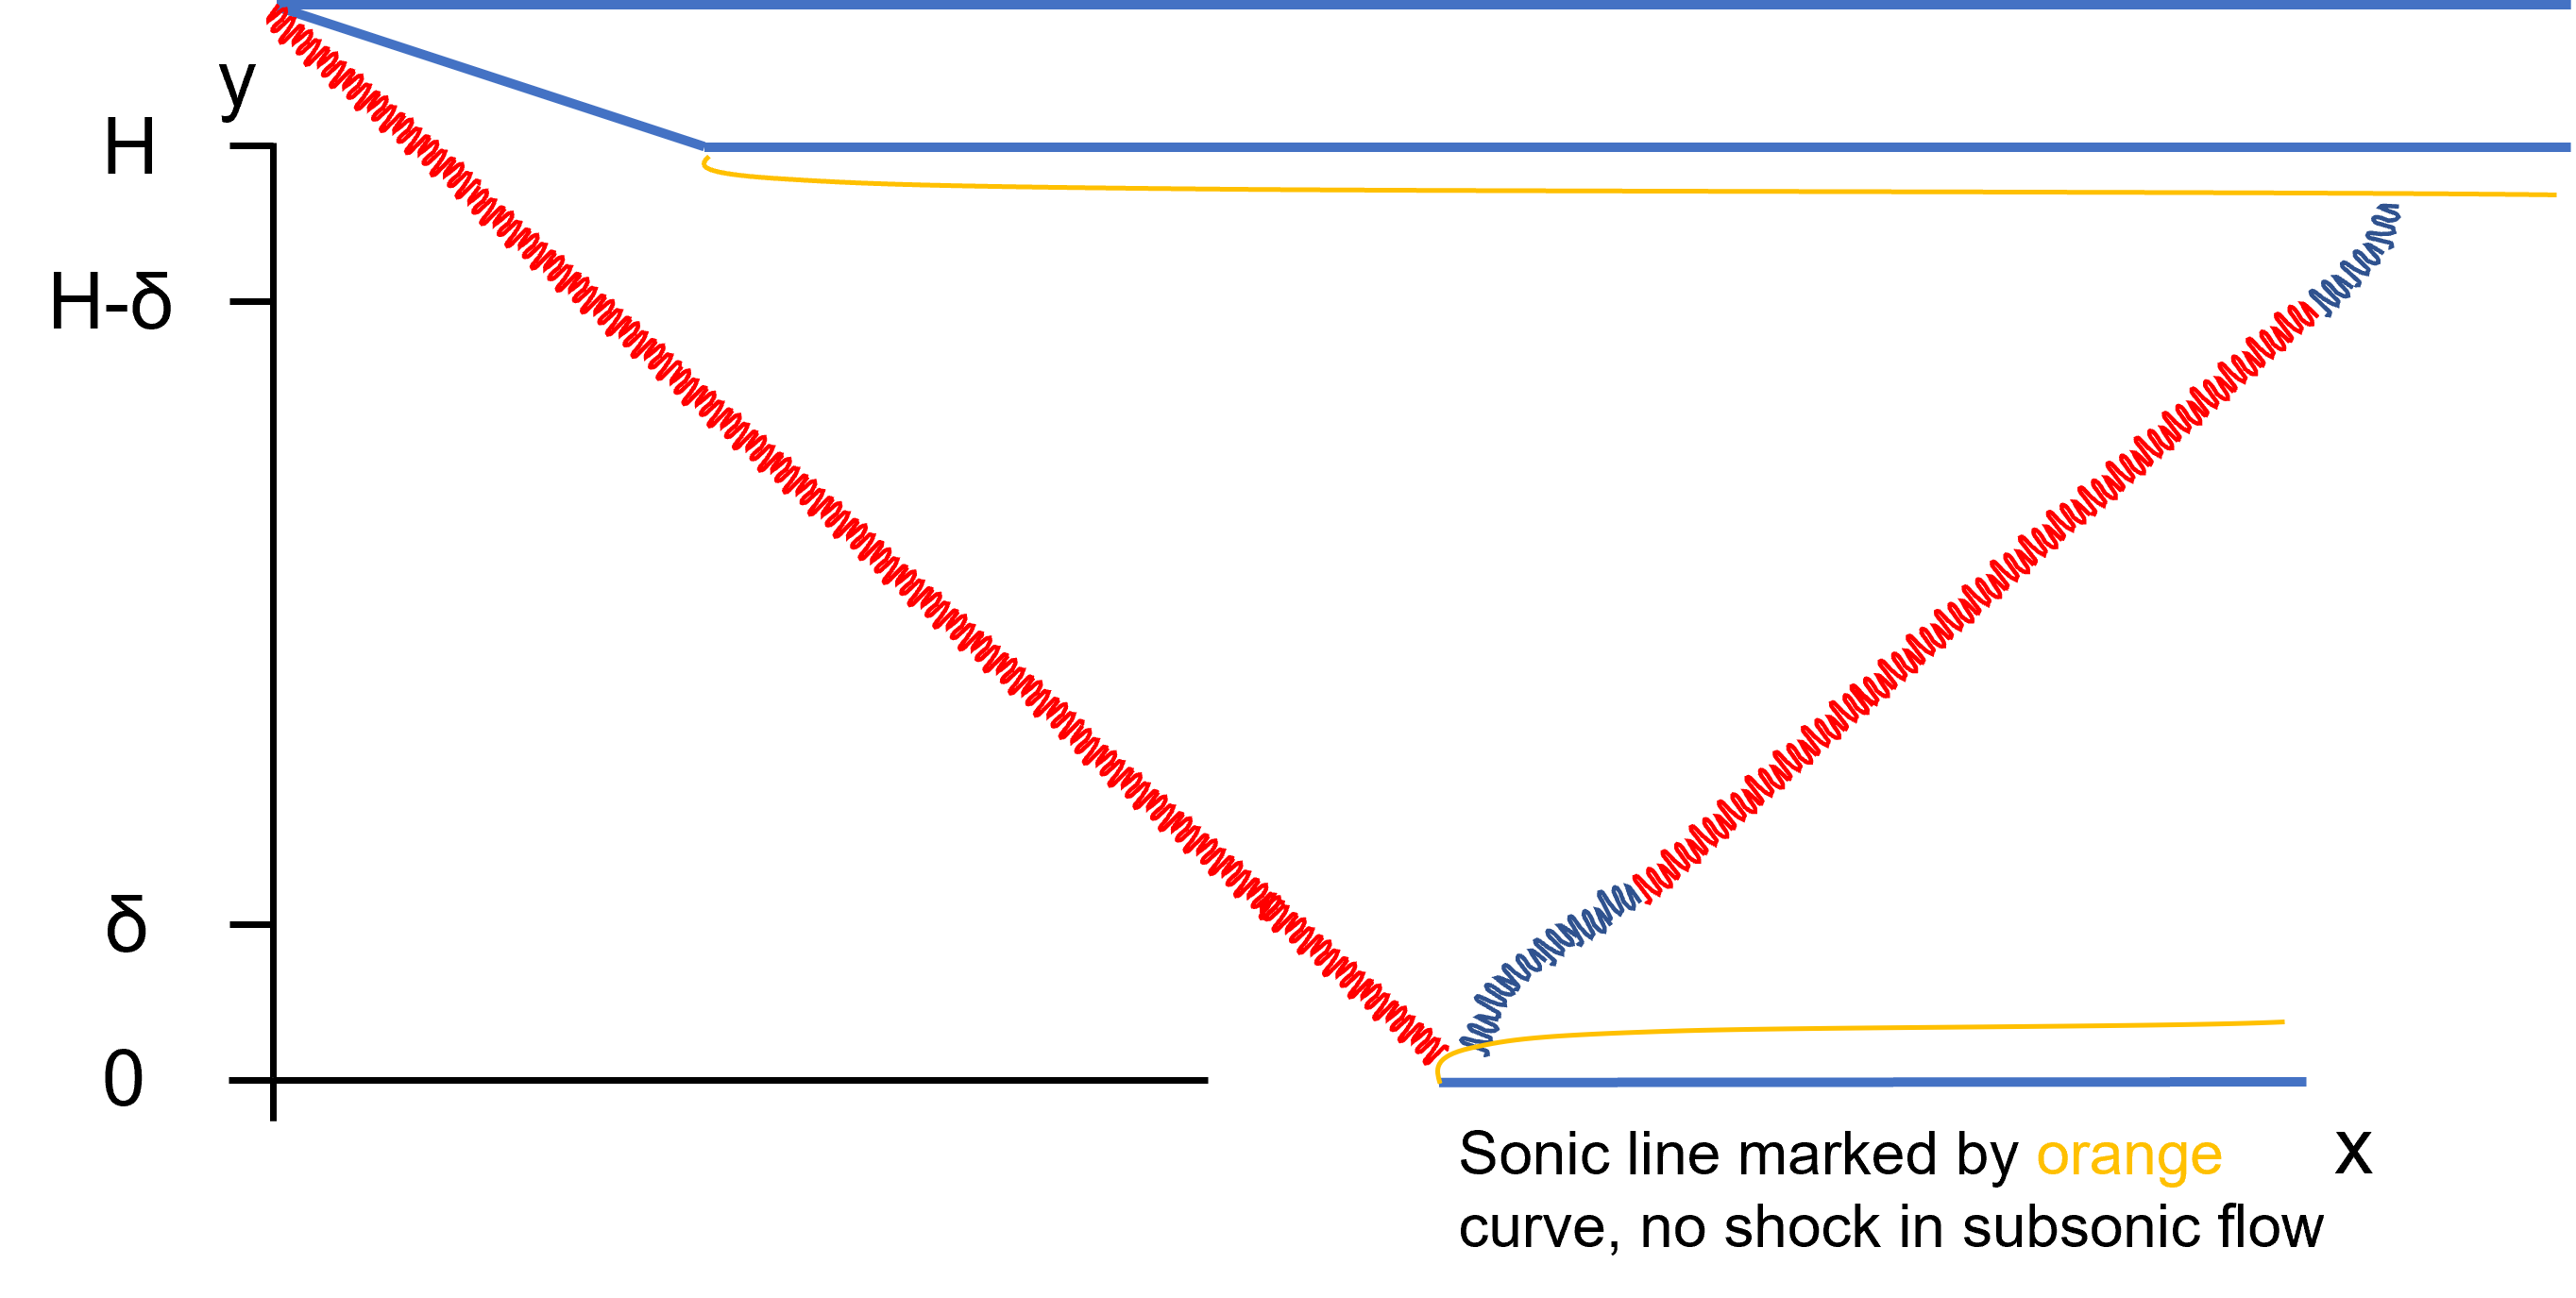
\includegraphics[scale=0.7]{../../images/problem_3/shock_inlet.png}
    \caption{Inlet with viscous effects}
    \label{viscous_inlet}
\end{figure}

\end{document}